\chapter{Localization Algorithm} \label{chap:pf}
This chapter presents the solution's implementation. As mentioned before, it is based on \acf{MCL}. The terminology used in this chapter builds upon the \acs{PF}'s introduction in Section~\ref{sec:fund_pf}.

First the reasons for choosing \acs{MCL} instead of another algorithm are outlined. Afterwards, an overview of the system's setup is provided. Next the algorithm's \emph{motion model} is described, followed by a detailed insight in the solution's \emph{measurement model}. In the end, the algorithm's implementation is described, which builds upon the motion and measurement model.


\section{Design Decision} \label{sec:algo_decision}
This section outlines the reasons for choosing \acl{MCL} instead of another algorithm, as introduced in Chapter~\ref{chap:fundamentals}.

As shown in Chapter~\ref{chap:ibeacons} and mentioned by \citet{IEEE:survey_wireless_indoor_pos}, wireless signals are heavily influenced by obstacles and their environment. According to \citet{wang:wlan} and \citet{siddiqi:experiments_mcl_wifi}, location accuracy can be drastically improved by additionally using map information and motion tracking. Thus, the main reason for choosing \ac{MCL} is the fact, that \acl{PF} is the only algorithm, which has the ability to combine the \acs{RSS}-based measurements to the beacons with motion tracking by additionally using map information. Triangulation, the proximity method, and the scene analysis approach are not able to improve their location estimation by combining motion tracking with \ac{RSS}-based measurements. \acl{KF} is the only algorithm which is also capable of using motion besides \ac{PF}. But according to \citet{wang:wlan}, ``map information is impossible to be integrated for tracking by \acs{EKF}''.

The second reason for choosing \acs{PF} is its ability to solve the \emph{global localization problem}. Thus, the algorithm can start determining the user's location without knowing the user's initial position. Furthermore, the algorithm is able to recover form failure state, i.e.\ if the estimated location is completely wrong, e.g. due to short-term sensor failure, it is able to detect and to recover from that state.

The third reason is the algorithm's advantage of taking uncertainties into account. Besides \ac{PF}, \ac{KF} is the only mentioned algorithm which is also capable of modeling uncertainties. As mentioned before, \acs{PF} is a non-parametric filter with the advantage of expressing a location estimation in the form of a multi-modal posterior belief. Whereas \ac{KF} is a parametric filter which is fixed to normal distributed position estimations. Furthermore, the \ac{PF}'s multi-modal belief can be visually illustrated very well and the users can benefit from this as shown in Figure~\ref{fig:pf_approx}.

The fourth reason are the, in Chapter~\ref{chap:intro} defined, requirements. By using \acs{PF}, based on \acs{RSS}-based measurements, less pre-deployment effort is required. Furthermore, the required infrastructure is of little complexity compared to other solutions outlined in Chapter~\ref{chap:fundamentals}, which reduces the maintenance effort and the initial and maintenance costs.

Besides the above mentioned reasons, \acl{PF} is an easy-to-implement algorithm. Furthermore, \ac{MCL} is a well-known and well-studied approach for landmark-based localization in robotics, as mentioned by \citet{thrun:prob_robo}.


\section{System Setup}
\begin{figure}[height=0.45\textheight]
	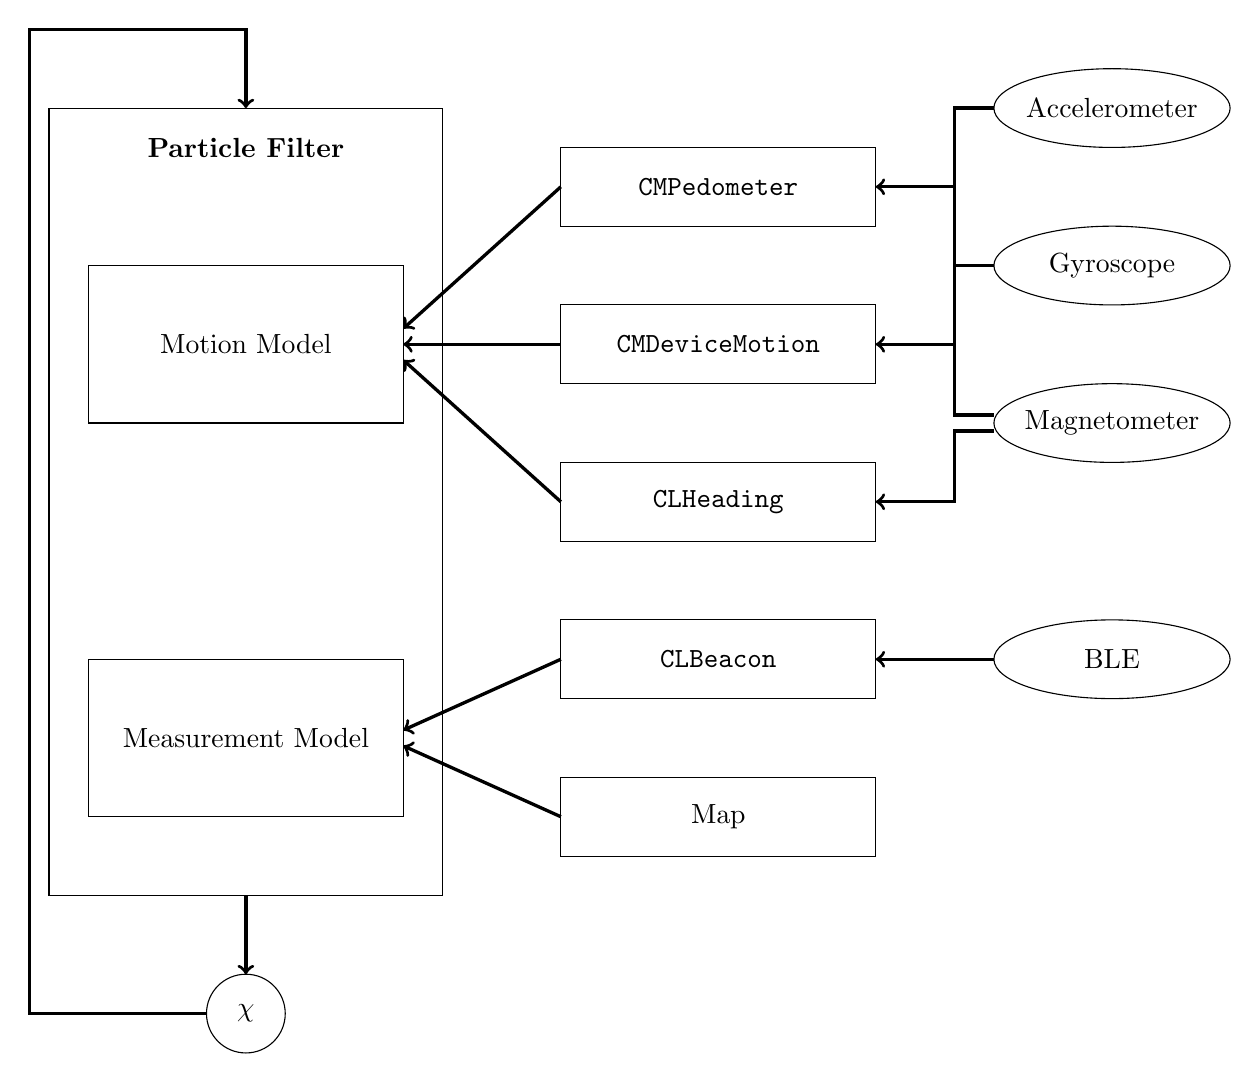
\begin{tikzpicture}
 %\draw[style=help lines] (0,0) grid (15,10);

 % sensors
 \node (A) at (13,9) {Accelerometer};
 \node (G) at (13,7) {Gyroscope};
 \node (M) at (13,5) {Magnetometer};
 \node (B) at (13,2) {\acs{BLE}};

 \draw (A) ellipse (1.5 and 0.5);
 \draw (G) ellipse (1.5 and 0.5);
 \draw (M) ellipse (1.5 and 0.5);
 \draw (B) ellipse (1.5 and 0.5);

 % Frameworks
 \node (CMP) at (8,8) {\texttt{CMPedometer}};
 \node (CMDM) at (8,6) {\texttt{CMDeviceMotion}};
 \node (CLH) at (8,4) {\texttt{CLHeading}};
 \node (CLB) at (8,2) {\texttt{CLBeacon}};
 \node (MAP) at (8,0) {Map};

 \draw (6,7.5) rectangle (10,8.5);
 \draw (6,5.5) rectangle (10,6.5);
 \draw (6,3.5) rectangle (10,4.5);
 \draw (6,1.5) rectangle (10,2.5);
 \draw (6,-0.5) rectangle (10,0.5);


 \draw[very thick] (11.5,9) -- ++(-0.5,0) -- ++(0,-2) -- ++(0.5,0) -- ++(-0.5,0) -- ++(0,-1.9) -- ++(0.5,0);
 \draw[->, very thick] (11,8) to (10,8);
 \draw[->, very thick] (11,6) to (10,6);


 \draw[->, very thick] (11.5,4.9) -- ++(-0.5,0) -- ++(0,-0.9) -- ++(-1,0);
 \draw[->, very thick] (11.5,2) to (10,2);

 % Particle Filter
 \draw (-0.5,-1) rectangle (4.5,9);
 \node (MM) at (2,8.5) {\textbf{Particle Filter}};

 % Motion Model
 \draw (0,5) rectangle (4,7);
 \node (MM) at (2,6) {Motion Model};

 \draw[->, very thick] (6,8) to (4,6.2);
 \draw[->, very thick] (6,6) to (4,6);
 \draw[->, very thick] (6,4) to (4,5.8);

 % Measurement Model
 \draw (0,0) rectangle (4,2);
 \node (MM) at (2,1) {Measurement Model};

 \draw[->, very thick] (6,2) to (4,1.1);
 \draw[->, very thick] (6,0) to (4,0.9);

 % Location
 \node (L) at (2,-2.5) {$\chi$};
 \draw (L) ellipse (0.5 and 0.5);
 \draw[->, very thick] (2,-1) -- ++(0,-1);
 \draw[->, very thick] (1.5,-2.5) -- ++(-2.25,0) -- ++(0,12.5) -- ++(2.75,0) -- ++(0,-1);

\end{tikzpicture}

	\caption{The solution's system setup including the used sensors and \acsp{API}.}
	\label{fig:algo_architecture}
\end{figure}

Before going into the detailed description of the solution, this section provides an overview of the system setup.

The implementation is written in Apple's new programming language \emph{Swift} (version 1.2), which is the successor of \emph{Objective-C}. The language is based on modern programming concepts, such as functional programming, tuples, generics, etc. Furthermore, Apple tries to remove unsafe code, such as not initialized variables, null-pointers, array overflows, etc.\ by defining the language's elements in a very concise and expressive syntax, and by adding new language constructs and types, such as the Optional type. The language compiles to native code by using LLVM compiler. Swift code can also call C and Objective-C code, which provides the possibility to use Swift in existing projects \citep{apple:swift}.

The system, depicted in Figure~\ref{fig:algo_architecture}, consists of the \ac{PF}, its components, and the used \acsp{API}. Furthermore, the figure depicts the sensors used by the \acsp{API}. As explained in Section~\ref{sec:fund_pf}, the algorithm uses two models, the \emph{Motion Model} and the \emph{Measurement Model}.

The Motion Model, described in Section~\ref{sec:algo_motion_model}, is on one hand, responsible for tracking the user's motion by combining different sources. On the other hand, it samples from the motion model. To implement this, the Core Motion framework's pedometer and device motion component are used, which both use the smartphone's accelerometer, gyroscope and magnetometer, as described in Chapter~\ref{chap:sensors}. Furthermore, the component uses the Core Location framework's compass, i.e.\ \texttt{CLHeading}, which uses the magnetometers data.

The Measurement Model, described in Section~\ref{sec:algo_measurement_model}, implements the \acs{PF}'s importance factor calculation. For that it uses Core Location's \texttt{CLBeacon} component, which provides the \acs{RSS}-based distances estimations to the beacons. It uses the smartphone's \acf{BLE} module, to receive the beacons' \ac{BLE} signals. Furthermore, the Measurement Model uses the building's map.

The \acl{PF}, described in Section~\ref{sec:algo_pf}, outputs the posterior, i.e.\ the position estimation represented by the particle set $\chi$. Furthermore, $\chi$ is passed to the function by its next iterative call.


\section{Motion Model}\label{sec:algo_motion_model}
The here presented solution's motion model component is responsible for three tasks: Firstly, for tracking the users motion, secondly, to determine if the user is stationary, and thirdly, to allow the \acs{PF} to sample from the motion model. The three tasks are prerequisites for the \acs{PF}'s implementation.

\subsection{Motion Tracking}
As mentioned in Chapter~\ref{chap:sensors}, \acl{CM} provides a component called \texttt{CMPedometer}, which estimates the traveled distance based on the steps a user has taken. In addition, \acl{CL} provides the smartphone's heading, based on the magnetic field, called \texttt{CLHeading}. Furthermore, \ac{CM}'s \texttt{CMDeviceMotion} provides the device attitude, which is calculated by using sensor fusion. The device's attitude can also be used to calculate the device's heading. By combining these three sources the user's motion can be tracked and a path can be constructed.

\subsubsection*{Heading}
\begin{lstlisting}[
  float,
  floatplacement=H,
  mathescape,
  captionpos=b,
  caption={Illustrates the calculation of the internal heading $\theta$, by combining $\theta_C$ and $\theta_A$, relative to the maps orientation $\theta_M$},
  label=lst:motionModelHeadingCalculation]
// instance variables
$\theta_{A_\text{current}}$, $\theta_{A_\text{last}}$ = nil
$\theta_{C_\text{last}}$ = nil

// combined internal heading
$\theta$ = 0.0

// called by CoreMotion if new heading is available
didMeasureDeviceMotionHeading($\theta_{A_t}$) {
  $\theta_{A_\text{current}} = \theta_{A_t} - \theta_M$
}

// called by CoreLocation if new heading is available
didMeasureCompassHeading($\theta_{C_t}$) {
  $\theta_{C_\text{current}} = \theta_{C_t} - \theta_M$

  if $\theta_{A_\text{latest}} \neq \text{nil}$ && $\theta_{A_\text{last}} \neq \text{nil}$ && $\theta_{C_\text{last}} \neq \text{nil}$ {
    $\Delta\theta_{A} = \theta_{A_\text{current}} - \theta_{A_\text{last}}$
    $\Delta\theta_{C} = \theta_{C_\text{current}} - \theta_{C_\text{last}}$

    $\theta_{A_\text{last}} = \theta_{A_\text{current}}$

    $\theta = \theta_{t-1} + \frac{\Delta\theta_{C} + \Delta\theta_{A}}{2}$
  } else {
    $\theta = \theta_{C_\text{current}}$
  }

  $\theta_{C_\text{last}} = \theta_{C_\text{current}}$
}
\end{lstlisting}


\begin{table}
	\begin{tabular}{c|ccc|c|ccc||c}
\textbf{$t$} & \textbf{$\theta_C$} & \textbf{$\theta_A$} & \textbf{$\theta_M$} & $\theta_{C_\text{current}}$ & $\theta_{C_\text{last}}$ & $\theta_{A_\text{current}}$ & $\theta_{A_\text{last}}$ & \textbf{$\theta$}\\
\hline
$t_0$ & $90.3$ & & $20.0$ & $70.3$ & & & & $70.3$\\
$t_1$ & & $78.2$ & $20.0$ & & $70.3$ & $58.2$ & &\\
$t_2$ & & $79.0$ & $20.0$ & & $70.3$ & $59.0$ & $58.2$ &\\
$t_3$ & $91.3$ & & $20.0$ & $71.3$ & $70.3$ & $59.0$ & $58.2$ & $71.2$\\
$t_4$ & & $79.7$ & $20.0$ & & $71.3$ & $59.7$ & $59.0$ &\\
$t_5$ & $92.3$ & & $20.0$ & $72.3$ & $71.3$ & $59.7$ & $59.0$ & $72.1$
\end{tabular}

	\caption{Example calculation of the internal heading~$\theta$ according to the algorithm depicted in Listing~\ref{lst:motionModelHeadingCalculation}.}
	\label{tab:motionModelHeadingCalculationExample}
\end{table}

As mentioned in Chapter~\ref{chap:sensors}, the heading provided by \texttt{CLHeading} can be influenced by magnetic fields other than the earth's magnetic field, which may cause wrong values. \texttt{CMDeviceMotion} uses sensor fusion instead of relying only on the magnetometer's values. Thus, it is not influenced by other magnetic fields. In contrast to the claims made by Apple's engineer \citet{apple:wwdc_2012_pham}, the values tend to drift away. Consequently, relying only on \texttt{CMDeviceMotion} is not sufficient. As a result, both sources are combined to determine the smartphone's heading.

Both frameworks provide their values asynchronously. \texttt{CLLocationManager} calls its delegate method if a certain threshold of the heading's change, set to $1^\circ$, exceeds. Whereas \acs{CM} calls its delegate periodically, every $\approx$\,0.02\,s. The high update rate would not be necessary for heading, but as mentioned earlier, \texttt{CMDeviceMotion} also includes \texttt{userAccleration}, which is used for the stationary detection, as shown later.

The \texttt{CMDeviceMotion} heading, further denoted as $\theta_A$, measured at time~$t$, is calculated from the rotation matrix, given by \texttt{CMDeviceMotion}'s \texttt{attitude}, as explained in Chapter~\ref{chap:sensors}. Due to its drift problem, only the change between two values, denoted as $\Delta\theta_A$, is used. For the absolute orientation, \texttt{CLHeading}'s \texttt{magneticHeading}, denoted as $\theta_C$, is used. Internally the motion tracking uses the heading $\theta$, which takes the map's orientation $\theta_M$ into account. $\theta$ is calculated if \acs{CL}'s heading filter is exceeded and thus, a new magnetic heading is provided. It is not updated if \acs{CM} provides a new $theta_A$, due to its high update frequency, which would result in many useless updates of $\theta$ with very small change.

Listing~\ref{lst:motionModelHeadingCalculation} illustrates the used algorithm to calculate the internally used heading~$\theta$. It combines the two heading sources for more robustness against influences of disturbing magnetic fields without the drift problem. Furthermore, Table~\ref{tab:motionModelHeadingCalculationExample} provides a calculation example for better understanding.



\subsubsection*{Motion Path Construction}
As explained in Chapter~\ref{chap:sensors}, \acs{CM} delivers every $\approx$\,2.5\,s a new \texttt{CMPedometer} object with the estimation of the user traveled distance~$d$. Besides the distance, the object contains the start date~$t_\text{start}$, which is the start date of the very first distance estimation. It is the same for all successive estimations. Additionally, it contains the end date~$t_\text{end}$. Thus, the user walked an estimated distance~$d$, beginning at $t_\text{start}$ and ending at $t_\text{end}$. During the walk, the user's direction $\theta$ changes several times at a certain point in time.

A user's motion path is stored as an array of motions~$u$. A motion consists of $u = (\theta, d, t_\text{start}, t_\text{end})^T$, the orientation~$\theta$ at the motions start date~$t_\text{start}$, the distance~$d$ in meters and the motions end date~$t_\text{end}$. $t_\text{start}$ and $t_\text{end}$ are not really necessary for constructing the estimated motion path, but are necessary for the later explained motion integration.

To calculate the motion~$u$ of a walked distance~$d$, the distance is split according to the timestamps corresponding to the smartphone's orientational changes, which occurred during the estimated distance. To do so, constant velocity over the distance~$d$ is assumed. Figure~\ref{fig:mm_path} illustrates the estimated path a user traveled in 2-dimensional space. The individual distances~$d_1$ and $d_2$, estimated by \acs{CM} are colored differently. By integrating the measured headings~$\theta_0, \ldots, \theta_4$, the path is split into motion~$u_0, \ldots, u_5$.

\begin{figure}
	\begin{tikzpicture}
\draw[->] (0,0) -- (8,0);
\draw[->] (0,0) -- (0,7);
\draw (8.5,0)node(y){$x$};
\draw (0,7.5)node(y){$y$};


\draw[blue] (1,6)--(5,6);
\draw (1,6.5)node(a){$\theta_0$};
\draw[blue] (3,6.5)node(b){$d_0$};
\draw(3,5.5)node(b){$u_0$};
%     \fill[red] (5,6) circle (2pt);

\draw[blue] (5,6)--(7,4);
\draw (5,6.5)node(c){$\theta_1$};
\draw(5.6,4.7)node(b){$u_1$};

\draw[blue] (7,4)--(7,3);
\draw (7.5,4)node(d){$\theta_2$};
\draw(6.5,3.5)node(b){$u_2$};

\draw[red] (7,3)--(7,1);
\draw (7,0.5)node(e){$\theta_3$};
\draw(6.5,2.0)node(b){$u_3$};

\draw[red] (7,1)--(3,1);
\draw[red] (5,0.5)node(b){$d_1$};
\draw(5,1.5)node(b){$u_4$};


\draw[red] (3,1)--(3,4);
\draw (3,0.5)node(e){$\theta_4$};
\draw(3.5,2.5)node(b){$u_5$};
\end{tikzpicture}

	\caption{Illustration of the motion path construction by integrating heading $\theta_0, \ldots, \theta_4$ into the two estimated distances $d_1, d_2$. $u_0, \ldots, u_5$ are the resulting motions.}
	\label{fig:mm_path}
\end{figure}


\subsection{Stationary Detection}\label{sec:algo_stationary}
As mentioned in Chapter~\ref{chap:sensors}, the \texttt{CMPedometer} component requires at the beginning $\approx$\,6\,--\,8\,steps to deliver the first distance estimation. During a walk it continuously updates the estimation every $\approx$\,2.5\,s. Due to the asynchronously incoming motion and beacon data, the filter cannot be run continuously with a fixed time interval, because the later discussed measurements need to be integrated at the right position on the user's walk. Thus, it is important to know whether or not the user is currently walking, i.e.\ is stationary or not.

\citet{wang:wlan} propose a system based on acceleration data to detect a user's steps by detecting the acceleration's zero-crossing. However, the system does not actually need to count the user's steps, which would require too much effort to get this information. Also, \citet{shanklin:embedded_sensors} use the user's acceleration to estimate the distance the user traveled. First they filter the values with a low-pass filter. Then they integrate the acceleration two times to get the distance. Thus, to detect if a user is stationary, one integration step would be sufficient to get the user's velocity. This requires a projection of the measured acceleration data into the global coordinate system as described by~\citet{shanklin:embedded_sensors}. Unfortunately, their solution works very unreliable. According to \citet{wang:wlan}, integration of acceleration data for distance estimation works only in theory, but not reliably in indoor environments. Furthermore, their proposed projection is based on \texttt{CMDeviceMotion}'s \texttt{attitude} property, which suffers from the drift problem as shown in Section~\ref{sec:sensor_eval}.

\begin{figure}[p]
	\begin{tikzpicture}
    \begin{axis}[trim axis left, trim axis right, width=0.9\textwidth, height=0.45\textheight,
        legend pos=north west,
        xlabel={Time (sec)},
    ylabel={User Acceleration ($ms^{-2}$)},
      legend entries={x, y, z},
      grid = major]
      \addplot [red, no marks] table[col sep=semicolon, x=timestamp, y=x] {csv/acceleration/acc.csv};
      \addplot [blue, no marks] table[col sep=semicolon, x=timestamp, y=y] {csv/acceleration/acc.csv};
      \addplot [green, no marks] table[col sep=semicolon, x=timestamp, y=z] {csv/acceleration/acc.csv};
  \end{axis}
\end{tikzpicture}

	\caption{Example data of the 3-axis \texttt{userAcceleration} provided by \acs{CM}'s \texttt{CMDeviceMotion} object. The user's two stationary phases are clearly depicted by the low amplitude. Remark: \texttt{userAcceleration} is without gravity.}
	\label{fig:mm_stationary_1}
\end{figure}

\begin{figure}[p]
	\begin{tikzpicture}
    \begin{axis}[trim axis left, trim axis right, width=0.9\textwidth, height=0.4\textheight,
    legend pos=north east,
        xlabel={Time (sec)},
        ylabel={User Acceleration ($ms^{-2}$)},
        legend entries={$\left\lVert a \right\rVert = \sqrt[2]{x^{2}+y^{2}+z^{2}}$, moving avg.\ of $\left\lVert a \right\rVert$},
      grid = major]
      \addplot [blue, no marks] table[col sep=semicolon, x=timestamp, y=norm] {csv/acceleration/vel.csv};
      \addplot [red, no marks] table[col sep=semicolon, x=timestamp, y=avgnorm] {csv/acceleration/vel.csv};
  \end{axis}
\end{tikzpicture}

	\caption{The euclidian norm of the 3-axis \texttt{userAcceleration} shown in Figure~\ref{fig:mm_stationary_1}, and its simple moving average with a window of 1\,s which corresponds to 50\,measurements.}
	\label{fig:mm_stationary_2}
\end{figure}

\citet{shanklin:embedded_sensors} considered also another solution for step detection, which uses the user's minimum acceleration. Steps are detected by using a threshold, that needs to be exceeded by the acceleration's Euclidian-Norm $\left\lVert a \right\rVert = \sqrt[2]{x^{2}+y^{2}+z^{2}}$. Figure~\ref{fig:mm_stationary_1} depicts a user's 3-axis acceleration during a walk with two clearly visible stops. The corresponding Euclidian-Norm is shown in Figure~\ref{fig:mm_stationary_2}. For the actual detection of the stationary and not stationary state, a simple moving average can be used. It is calculated over the last 50 values which correspond to 1\,s using a update frequency of 0,02\,s. If the user walks the simple moving average exceeds a threshold of 0.1\,$ms^{-2}$.

The solution's advantage is, that it is quite easy to implement and does not need a projection of the user's acceleration data. As a result, the later discussed integration of measurements, i.e.\ the importance factoring can be delayed when the user starts to walk until \acs{CM} provides a distance estimation.
 
%\begin{equation} \label{eq:a}
%	\left\lVert a \right\rVert = \sqrt[2]{x^{2}+y^{2}+z^{2}}
%\end{equation}


\subsection{Sample Motion}\label{sec:algo_sample_motion}
As described in Section~\ref{sec:fund_mcl}, \acs{MCL} has a \texttt{sample\_motion\_model} function to sample from the motion model, i.e.\ to apply a motion $u$ to a state hypothesis~$x^{[m]}_{t-1}$ by taking the motion's uncertainties into account, as shown by Equation~\ref{eq:sample_motion}.

\begin{equation}\label{eq:sample_motion}
	x^{[m]}_t = \left(
    \begin{array}{c}
      x_t\\
      y_t\\
      \theta_t
    \end{array}
  \right) = \left(\begin{array}{c} x_{t-1} + \cos(\theta_u + \theta_{\text{noise}})\cdot (d_u + d_\text{noise}) \\ y_{t-1} + \sin(\theta_u + \theta_{\text{noise}})\cdot (d_u + d_\text{noise}) \\ \theta_u + \theta_{\text{noise}}
    \end{array}
  \right)
\end{equation}

\noindent The new state hypothesis is denoted as~$x^{[m]}_t$. A state is defined as~$x^{[m]} = (x, y, \theta)^T$, where $x$ and $y$ denote the position in 2-dimensional space and $\theta$ the user's orientation. $d_u$ and $\theta_u$ are the distance and heading of motion~$u$. The added noise~$d_\text{noise}$ and $\theta_\text{noise}$ are the translational and rotational uncertainties, modeled as Gaussians. First, the uncertainties, determined during the sensor evaluation shown in Section~\ref{sec:sensor_eval} were used, but as usual, they do not fit best. By trying different values the following better fitting values were derived.

\begin{equation}\label{eq:sigma_d}
	d_\text{noise} = NDF(\mu_\text{trans}, \sigma_\text{trans}) ,
	\quad \mu_\text{trans} = 0 ,
	 \quad \sigma_{\text{trans}} = \max(0.3, 0.3 \cdot d_u)
\end{equation}

\begin{equation}\label{eq:mu_d}
	\theta_\text{noise} = NDF(\mu_\text{rot}, \sigma_\text{rot}), \quad
	\mu_\text{rot} = 0 , \quad
	\sigma_\text{rot} = 20^{\circ}
\end{equation}

\noindent $d_\text{noise}$ depends on the motions distance~$d_u$, shown in Equation~\ref{eq:sigma_d}, whereas $\theta_\text{noise}$ uses constant parameters, shown in Equation~\ref{eq:mu_d}. Due to the lack of a built-in algorithm to sample from a Gaussian distribution the \texttt{sample\_normal\_distribution} algorithm proposed by \citet[p.~124]{thrun:prob_robo}, is used.


\section{Measurement Model}\label{sec:algo_measurement_model}
The measurement model component is responsible for the calculation of the importance factor~$w^{[m]}$ for a given state hypothesis~$x^{[m]}_t$ by taking the measurements~$z_t$, its uncertainties, and the \texttt{map} into account. The \texttt{map} represents the environment, i.e.\ the building in form of a simple occupancy grid.

The algorithm depicted in Listing~\ref{lst:measurementModelImportanceFactorCalculation} illustrates the calculation of the importance factor \texttt{weight} of one state hypothesis. If the state is out of the map's boundaries or the position is not free, e.g.\ the map contains an obstacle at this position, the weight for the state is set to~0.0. If the states is valid, an importance factor~$w$ for each of the measurements, i.e.\ for each distance estimation between the smartphone and the received beacons, is calculated.

\begin{lstlisting}[
  float,
  floatplacement=H,
  mathescape,
  captionpos=b,
  caption={Algorithm to calculate the importance factor $w$ of a state hypothesis $x$ by taking the measurements $z$ and the \texttt{map} into account.},
  label=lst:measurementModelImportanceFactorCalculation]
measurement_model($z = \{z_0, z_1, z_{k-1}\}$, $x$, map) {
  $\text{weight} = 0.0$

  if position $x$ on map && $x$ is free {

    for $z_i$ in $z$ {

      $z_{i_\text{dist}}$ = measured distance between phone and beacon
      $z_{i_\text{pos}}$ = beacons position on map

      $\mu_d$ = euclidian distance between $x$ and $z_{i_\text{pos}}$
      $\sigma_d = 0.25 \cdot z_{i_\text{dist}}$

      $w$ = PDF($z_{i_\text{dist}}$, $\mu_d$, $\sigma_d$)

      $\text{weight}$ = $\text{weight} \cdot w \cdot 10.0$
    }
  }
  return $\text{weight}$
}
\end{lstlisting}


To calculate~$w$, the euclidian distance between the state hypothesis~$x$, i.e.\ the particle, and  the beacon~$z_{i_\text{pos}}$ need to be determined. It is the mean value~$\mu_d$ required by the \ac{PDF}. The \ac{PDF}'s standard deviation~$\sigma_d$ depends on the distance~$z_{i_\text{dist}}$ between smartphone and the beacon. By trying different values, $\frac{1}{4}$ of $z_{i_\text{dist}}$ seems to fit best. The weight is then calculated by the \ac{PDF}(Listing~\ref{lst:measurementModelImportanceFactorCalculation}, Line 16). It is important to note, that only measurements with $z_{i_\text{dist}} < 5\text{m}$ are taken into account. Larger values are sorted out and not passed to the \texttt{measurement\_model} function, because estimated distances to a beacon larger than 5\,m are very unreliable, as shown in Section~\ref{sec:beacon_eval}.

Finally, the weights\,$w$ of each measurement are multiplied with each other, which is the importance factor~\texttt{weight} of this state hypothesis~$x$, i.e.\ particle. The reason for adding the additional factor of~10 for each subsequent \texttt{weight} is that otherwise the \texttt{weight}'s order of magnitude depends on the count of beacons. Of course, this only works because usually $0.1 \leq w < 1$. Table~\ref{tab:measurementModelWeightFactorIllustration} illustrates the exponential decline of the \texttt{weight} by increasing beacon count~$k$. For the illustration, all subsequent weights~$w$ of their importance factor~\texttt{weight} have the same value w\,=\,0.1. If the additional factor of~10 is added the beacon count is irrelevant for the weight's magnitude. Of course, during one run of the \acl{PF} the weight's magnitude is irrelevant, but to compare the sums of all importance factors over time, as used for the in Section~\ref{sec:algo_recovery} discussed recovery, this is very important.

\begin{table}
	\subfloat[Without additional factor]{
\begin{tabular}{ccl}
\textbf{$k$} & \textbf{$w$} & \texttt{weight}\\
\hline
$1$ & $0.1$ & $0.1^1 = 0.1$\\
$2$ & $0.1$ & $0.1^2 = 0.01$\\
$3$ & $0.1$ & $0.1^3 = 0.001$\\
$9$ & $0.1$ & $0.1^9 = 1 \cdot 10^{-9}$
\end{tabular}
}
\subfloat[With additional factor]{
\begin{tabular}{ccl}
\textbf{$k$} & \textbf{$w$} & \texttt{weight}\\
\hline
$1$ & $0.1$ & $(0.1 \cdot 10)^1 = 1$\\
$2$ & $0.1$ & $(0.1 \cdot 10)^2 = 1$\\
$3$ & $0.1$ & $(0.1 \cdot 10)^3 = 1$\\
$9$ & $0.1$ & $(0.1 \cdot 10)^9 = 1$
\end{tabular}
}

	\caption{Illustration of the importance factor's~\texttt{weight} exponential decline by increasing beacon count~$k$ if no additional factor is added.}
	\label{tab:measurementModelWeightFactorIllustration}
\end{table}


\section{\acl{PF}}\label{sec:algo_pf}
The \acl{PF} is the solution's heart, which is responsible for the position estimation by combining the before mentioned components. In this section first the \emph{initial generation of the particle set} is explained. Then two functions, named \texttt{integrateMotions} and \texttt{filter}, which are often called by the actual \ac{PF} implementation are introduced. Afterwards the \ac{PF}'s implementation is explained. In the end the \emph{kidnapping problem's} solution, i.e.\ the recovery's implementation is presented.


\subsection{Initial Particle Distribution}\label{sec:algo_initial}

\begin{figure}
\includegraphics[height=0.7\textwidth]{figures/algo_particle_generation}
\caption{Example of the initial posterior belief, i.e.\ the initial particle set. Particles are shown as red arrows, the beacons as blue filled circles. The large black circle is the $1\sigma$-ellipse introduced in Section~\ref{sec:algo_locEstimation}.}
\label{fig:pf_initialDist}
\end{figure}

Before the \ac{PF} can start to continuously run the initial posterior belief~$\chi_0$, i.e.\ the particle set, needs to be generated. Tests showed, that a static particle set size of 200\,particles is sufficient. As mentioned in Chapter~\ref{chap:ibeacons}, each of the beacons can be uniquely identified by combining the beacon's three identifiers. In addition, their position on the map, i.e.\ the local coordinate system, is known. Consequently, this information can be used to specifically distribute the initial particles around the received beacons. This is a huge advantage instead of uniformly distributing them on the map's free space. For that reason, the implementation starts searching for beacons and then waits until \ac{CL} reports the first ranged beacons. Then, the particles are distributed in a circle around the beacons with the radius of the estimated distance to that beacon. To take the distance estimation's uncertainty into account each distance of a particle to its beacon gets added some Gaussian noise with $\mu$\,=\,0 and $\sigma$\,=\,0.2\,$\cdot$\,d, which depends on the estimated distance~d. A particle's orientation~$\theta$ is a uniformly distributed random value within~[0,~2$\pi$).

Additionally, the amount of particles distributed around a beacon depends on the estimated proximity. 50\,\% of the particle set size are distributed around the particular beacon, which is most probably closest to the smartphone according to the beacons proximity, i.e.\ the estimated distance between smartphone and beacon. 25\,\% are distributed around the second closest beacon, 12.5\% around the third closest beacon, and so on. The beacon which's proximity is furthest from the smartphone, gets the remaining particles.

Figure~\ref{fig:pf_initialDist} shows a screenshot of the implemented iOS app depicting the initial particle set. The particles are depicted as small red arrows, the beacons as blue filled circles. The black large circle shows the $1\sigma\text{-ellipse}$, which is explained in Section~\ref{sec:algo_locEstimation}.


\subsection{Motion Integration}
The \texttt{integrateMotion} function, shown in Listing~\ref{lst:algorithmIntegrateMotion}, is a helper function to reduce the complexity of the later introduced algorithm. The function's arguments are the current particle set~$\chi_{t-1}$ and the motion~$u_t$ which it applies to each particle. Thus, it samples from the motion model as discussed in Section~\ref{sec:algo_sample_motion}. In the end it returns the new particle set~$\chi_t$.

\begin{lstlisting}[
  float,
  floatplacement=H,
  mathescape,
  captionpos=b,
  caption={Helper function to apply the motion $u_t$ to the particle set $\chi_{t-1}$, by sampling from the motion model.},
  label=lst:algorithmIntegrateMotion]
integrateMotion($\chi_{t-1}$, $u_t$) {

  $\bar{\chi}_t = \emptyset$

  for $m = 1$ to $M$ {
    $x^{[m]}_t$ = sample_motion_model($u_t$, $x^{[m]}_{t-1}$)
  }

  return $\bar{\chi}_t$
}chi\end{lstlisting}



\subsection{Filtering}
The \texttt{filter} function is another helper function, which is responsible for the \emph{importance factoring} and the \emph{resampling}, depicted in Listing~\ref{lst:algorithmSimpleFilter}. The function's arguments are the particle set~$\chi_{t-1}$, the measurements~$z_t$, and the \texttt{map}. Then it determines the importance factor of each particle as explained in Section~\ref{sec:algo_measurement_model}. Afterwards, the resampling takes place to transform the old distribution into the new posterior distribution as described in Section~\ref{sec:fund_pf}. The solution uses \emph{roulette wheel resampling}, which is a common resampling method based on \emph{independent sampling} proposed by \citet[p. 108--111]{thrun:prob_robo}.

The shown implementation is the basic implementation which does not solve the kidnapping problem. To better understand the implementation, the \acs{PF}'s complexity was reduced by first showing a simplified filter function, which neglects the recovery. Later in the chapter the shown \texttt{filter} function is enhanced to explain the implemented recovery feature.

\begin{lstlisting}[
  float,
  floatplacement=P,
  mathescape,
  captionpos=b,
  caption={Helper function for the \acs{PF}'s importance factoring and resampling.},
  label=lst:algorithmSimpleFilter]
filter($\chi_{t-1}$, $z_t$, map) {

  $\bar{\chi}_t = \emptyset$

  // importance factoring
  for $m = 1$ to $M$ {
    $w^{[m]}_t$ = measurement_model($z_t$,$x^{[m]}_t$, map)
    add $\langle x^{[m]}_t, w^{[m]}_t \rangle$ to $\bar{\chi}_t$
  }

  $\chi_t = \emptyset$

  \\ resampling
  while size of $\chi_t$ less $M$ {
    draw $i$ with probability $\propto w^{[m]}_t$
    add $x^{[i]}_t$ to $\chi_t$
  }

  return $\chi_t$
}return\end{lstlisting}



\subsection{\acl{PF}}

\begin{lstlisting}[
  float,
  floatplacement=H,
  mathescape,
  captionpos=b,
  caption={Shows our \acs{PF}'s implementation and the used instance variables. To reduce the complexity the code is split up into three parts, shown in figure~\ref{lst:algo_pf_1}, \ref{lst:algo_pf_2} and \ref{lst:algo_pf_3}.},
  label=lst:algorithmParticleFilter]
// instance variables
u_buffer // list of not jet integrated motions $u_t$
$u_\text{latest}$ // stores the latest motion
z_buffer // list of not jet integrated measurements $z^{[k]}_t$
map // occupancy grid and landmarks

particleFilter($\chi_{t-1}$) {

  $\bar{\chi}_t = \chi_{t-1}$

  $\bar{\chi}_t$ = PART_1($\bar{\chi}_t$)

  $\bar{\chi}_t$ = PART_2($\bar{\chi}_t$)

  $\bar{\chi}_t$ = PART_3($\bar{\chi}_t$)

  return $\chi_t$
}
\end{lstlisting}


After explaining all prerequisites this section provides a detailed insight into the solution's \acl{PF} implementation. To reduce complexity the \acs{PF}'s code is divided into three logical parts, shown in Listing~\ref{lst:algorithmParticleFilter_1}, \ref{lst:algorithmParticleFilter_2} and \ref{lst:algorithmParticleFilter_3}. Listing~\ref{lst:algorithmParticleFilter} indicates their call order. It also contains several instance variables, which are accessible from the three parts.

The \texttt{particleFilter} function is continuously called every $\approx$\,1\,s if new measurements are available. To remember, \ac{CL} calls its delegate to update the ranged beacons whether it received a beacon's signal or not. Consequently, when the function gets called, the latest measurements are always available and ready for processing. The function takes the particle set~$\chi_{t-1}$ as argument and returns the new particle set~$\chi_t$.

The implementation uses a static particle set size of 200\,particles. Tests showed, that 200\,particles are sufficient and increasing the particle set does not really improve the estimation. The \texttt{particleFilter} function requires for one execution on average $\approx$\,10\,ms. Thus, a dynamic particle set size to safe processing power is also not required.


\subsubsection*{Instance Variables}
As mentioned, the motions and measurements are delivered asynchronously by their frameworks. The motion model's implementation already reduces this problem by combining the two headings and the estimated walked distance into one motion. Thus, the \acs{PF}'s implementation has just to deal with two asynchronous sources. To overcome the asynchrony, the motions~$u$ and measurements~$z$ are buffered in two ascending ordered lists, the \texttt{u\_buffer} and \texttt{z\_buffer}, according to their timestamps. The stored motions and measurements are provided by the motion model and the measurement model, and defined as mentioned in Section~\ref{sec:algo_motion_model} and Section~\ref{sec:algo_measurement_model}. The instance variable~$u_\text{latest}$ stores, as the name already implies, the latest motion that was calculated by the motion model. The \texttt{map} variable stores the environment's map in the form of an occupancy grid and the beacons' positions together with their unique identifiers.


\subsubsection*{\acl{PF} Function --- Part 1}
\begin{figure}[height=0.3\textheight]
	\subfloat[Case: $u.{t_\text{end}} < z.t$]{
  \begin{tikzpicture}
    \draw[->] (0,1) -- (6,1);
      \draw (6.5,1)node(y){$t$};

      \draw[blue] (1,2)--(3,2);
      \draw[blue] (2,2.5)node(a){$u_0$};

      \draw[red, dashed] (3,2)--(5,2);
      \draw[red] (4,2.5)node(a){$u_1$};

      \draw (4,1)--(4,0.5);
      \draw (4,0)node(a){$z_0$};
  \end{tikzpicture}
  \label{fig:algo_pf_1_1}
}
\subfloat[Case: $u.{t_\text{end}} = z.t$]{
  \begin{tikzpicture}
    \draw[->] (0,1) -- (6,1);
      \draw (6.5,1)node(y){$t$};

      \draw[blue] (1,2)--(3,2);
      \draw[blue] (2,2.5)node(a){$u_0$};

      \draw[red, dashed] (3,2)--(5,2);
      \draw[red] (4,2.5)node(a){$u_1$};

      \draw (3,1)--(3,0.5);
      \draw (3,0)node(a){$z_0$};
  \end{tikzpicture}
  \label{fig:algo_pf_1_2}
}

\subfloat[Case: $u.{t_\text{start}} < z.t < u.{t_\text{end}}$]{
  \begin{tikzpicture}
    \draw[->] (0,1) -- (6,1);
      \draw (6.5,1)node(y){$t$};

      \draw[blue] (1,2)--(3,2);
      \draw[blue] (2,2.5)node(a){$u_0$};

      \draw[red, dashed] (3,2)--(5,2);
      \draw[red] (4,2.5)node(a){$u_1$};

      \draw (2,1)--(2,0.5);
      \draw (2,0)node(a){$z_0$};
  \end{tikzpicture}
  \label{fig:algo_pf_1_3}
}
\subfloat[Case: \texttt{else}]{
  \begin{tikzpicture}
    \draw[->] (0,1) -- (6,1);
      \draw (6.5,1)node(y){$t$};

      \draw[blue] (1,2)--(3,2);
      \draw[blue] (2,2.5)node(a){$u_0$};

      \draw[red, dashed] (3,2)--(5,2);
      \draw[red] (4,2.5)node(a){$u_1$};

      \draw (0.5,1)--(0.5,0.5);
      \draw (0.5,0)node(a){$z_0$};
  \end{tikzpicture}
  \label{fig:algo_pf_1_4}
}

	\caption{Illustration of the four if-cases shown in Listing~\ref{lst:algorithmParticleFilter_1}.}
	\label{fig:algo_pf_1}
\end{figure}

The algorithm's first part, shown in Listing~\ref{lst:algorithmParticleFilter_1}, consists of basically one loop, which tries to integrate the buffered motions and filter with the buffered measurements at the right point in time. The loop is executed as long as both buffers are not empty. The four if-cases are visualized in Figure~\ref{fig:algo_pf_1}. In each example, the \texttt{u\_buffer} contains two motions~$u_0, u_1$, and the \texttt{z\_buffer} contains one measurement~$z_0$. Each subfigure illustrates only the loop's first iteration. Thus, $u_1$ is not relevant during this iteration.

\begin{lstlisting}[
  float,
  floatplacement=H,
  mathescape,
  captionpos=b,
  caption=Part 1,
  label=lst:algorithmParticleFilter_1]
PART_1($\chi_{t-1}$) {

  $\bar{\chi}_t = \chi_{t-1}$

  while u_buffer isNotEmpty && z_buffer isNotEmpty {
    $u$ = u_buffer.first
    $z$ = z_buffer.first
    if $u.{t_\text{end}}$ < $z.t$ {
      $\bar{\chi}_t$ = integrateMotion($\bar{\chi}_t$, $u$)
      u_buffer.remove($u$)
    } else if $u.{t_\text{end}} = z.t$ {
      $\bar{\chi}_t$ = integrateMotion($\bar{\chi}_t$, $u$)
      $\bar{\chi}_t$ = filter($\bar{\chi}_t$, $z$, map)
      u_buffer.remove($u$)
      z_buffer.remove($z$)
    } else if $u.{t_\text{start}} < z.t$ && $z.t < u.{t_\text{end}}$ {
      split $u$ at timestamp $z.t$ in $u_1$ and $u_2$
      $\bar{\chi}_t$ = integrateMotion($\bar{\chi}_t$, $u_1$)
      $\bar{\chi}_t$ = filter($\bar{\chi}_t$, $z$, map)
      u_buffer.remove($u$)
      insert $u_2$ at beginning of u_buffer
      z_buffer.remove($z$)
    } else {
      $\bar{\chi}_t$ = filter($\bar{\chi}_t$, $z$, map)
      z_buffer.remove($z$)
    }
  }

  return $\bar{\chi}_t$
}
\end{lstlisting}


\begin{itemize}
\item{Case 1} (Figure~\ref{fig:algo_pf_1_1}): If a motion ends before the measurement was taken ($u.{t_\text{end}} < z.t$) the motion is integrated and the measurement is reserved for the next iteration.

\item{Case 2} (Figure~\ref{fig:algo_pf_1_2}): If a measurement is taken exactly at the end of a motion ($u.{t_\text{end}} = z.t$) the motion is integrated. Afterwards, the set is filtered with the measurement.

\item{Case 3} (Figure~\ref{fig:algo_pf_1_3}): If a measurement is taken during a motion ($u.{t_\text{start}} < z.t < u.{t_\text{end}}$) the motion needs to be divided. The first sub motion is then integrated into the particle set. Afterwards it is filtered with the measurement. The second sub motion is stored in the buffer at the first place to be processed during the loop's next iteration.

\item{Case 4} (Figure~\ref{fig:algo_pf_1_4}): If the measurement was taken before the motion ($u.{z.t < t_\text{start}}$ / \texttt{else}) the filter is executed without integrating the motion. The motion is kept back for the next iteration.
\end{itemize}

\noindent If one of the buffers is empty the algorithm continues with the function's second part.


\subsubsection*{\acl{PF} Function --- Part 2}
If, after executing the first part, motions are still buffered, these motions are integrated in this part. The reason for the remaining motions is that the \texttt{particleFilter} function is also called if no measurements are received as mentioned at the beginning. The reason why they can be integrated without current measurements is that they are definitely older than the not yet occurred measurements and thus there is no reason to keep them back.

After integrating a motion the filter method is called. The filtering is executed without an actual measurement. Thus, only the map's occupancy grid is used to calculate the particle's importance factors. Consequently, particles that are moved onto an occupied position are sorted out.

The purpose of not waiting for the next measurement to integrate the remaining motions is on one hand, that if the user is out of the beacons range, the motion is still integrated. Thus, the particles on the view are still moving according to the users motion. On the other hand the algorithm's performance does not get worse, because \texttt{u\_buffer} does not collect motions of several time steps that need to be integrated at once.

\begin{lstlisting}[
  float,
  floatplacement=H,
  mathescape,
  captionpos=b,
  caption={Part 2 of the solution's \texttt{particleFilter} function shown in Listing~\ref{lst:algorithmParticleFilter}.},
  label=lst:algorithmParticleFilter_2]
PART_2($\chi_{t-1}$) {

  $\bar{\chi}_t = \chi_{t-1}$

  // integrate remaining motions and filter with map
  while u_buffer isNotEmpty {
    $u$ = u_buffer.first
    $z = \emptyset$
    $\bar{\chi}_t$ = integrateMotion($\bar{\chi}_t$, $u$)
     u_buffer.remove($u$)

     // empty measurements
     $\bar{\chi}_t$ = filter($\bar{\chi}_t$, $z$, map)
  }

  return $\bar{\chi}_t$
}
\end{lstlisting}



\subsubsection*{\acl{PF} Function --- Part 3}
The first two parts are important for integrating and filtering while a person is walking. But integrating measurements if a person is stationary can drastically improve the estimated location, as shown in Chapter~\ref{chap:evaluation}. Thus, the received measurements are directly integrated instead of buffered, as shown in Listing~\ref{lst:algorithmParticleFilter_3}. Furthermore, by applying the measurements directly the user sees without a long delay how the estimated position changes.

To be able to integrate them directly the algorithm needs to be sure that the user is stationary. As mentioned in Chapter~\ref{chap:sensors}, \acs{CL} has the problem of requiring 6\,--\,8\,steps to recognize that a person is walking, i.e.\ until it delivers this information. Consequently, if a user is stationary and starts to walk, the measurements collected during the first steps need to be buffered until the motion data is available, otherwise the measurements would be integrated at the wrong position. The second important information is to know, that a person is now stationary and no further motions are being delivered. Only then the measurements can be directly integrated without delay.

The latter problem can be solved easily. Motions are delivered every $\approx$\,2.5\,s. Thus, if the difference between now and the latest motion~$u_\text{latest}$ is at least 2.7\,s, \acs{CM} does not deliver any new motion until the person starts to walk again. 2.7\,s was chosen, because the 2.5\,s are an approximate value. Besides that, the \texttt{particleFilter} function is only invoked every $\approx$\,1\,s. Thus, no additional delay is created.

To be able to buffer the measurements during the first steps when the user starts to walk again, the solution presented in Section~\ref{sec:algo_stationary} is used. Due to the solution's simple moving average over the last $\approx$\,1\,s it detects within $\approx$\,1\,s if a user is stationary or not. Thus, if the user is not stationary, the motion integration is not executed and the values are kept in the buffer.

Furthermore, tests showed, that additionally integrating a small Gaussian distributed random motion with $\sigma$\,=\,0.3\,m helps to faster improve the location accuracy. If a person is stationary, the person's orientation does not matter. Consequently, also the motion's orientation~$\theta$ is set to an uniformly distributed random value between [0,~2$\pi$). Using a random orientation has the advantage that the particles can move in any direction.

\begin{lstlisting}[
  float,
  floatplacement=H,
  mathescape,
  captionpos=b,
  caption=Part 3,
  label=lst:algorithmParticleFilter_3]
PART_3($\chi_{t-1}$) {

  $\bar{\chi}_t = \chi_{t-1}$

  $\Delta t$ = currentDate - $u_\text{latest}.t_\text{end}$ // in seconds

  if motionModel.deviceIsStationary && $\Delta t \le 2.7$  {
    $u$ = motion with distance $0.0$
    $z$ = z_buffer.first

    $\bar{\chi}_t$ = integrateMotion($\bar{\chi}_t$, $u$)
    $\bar{\chi}_t$ = filter($\bar{\chi}_t$, $z$, map)
    z_buffer.remove($z$)
  }

  return $\bar{\chi}_t$
}
\end{lstlisting}



\subsection{Recovery}\label{sec:algo_recovery}
The implemented recovery feature has two purposes. First, it can happen that all particles are moving out of bounds, and thus are filtered out. Second, if the particles are on a totally wrong position, which can happen if the user walked too softly. Thus the pedometer could not recognize the user's steps. It can also happen that the orientation does not fit the actual one. For instance, the user's phone does not points straight forward during the walk.

\begin{lstlisting}[
  float,
  floatplacement=H,
  mathescape,
  captionpos=b,
  caption={The solution's enhanced filter function including recovery based on Listing~\ref{lst:algorithmSimpleFilter}.},
  label=lst:algorithmFilter]
// instance variable
weightSums // array that stores the last 3 weight sums

filter($\chi_{t-1}$, $z_t$, map) {

  $\bar{\chi}_t = \emptyset$

  if size of weightSum == 3 && avg.\ weightSums < 1.0 {
    add $0.2\%$ additional random particles to $\chi_{t-1}$
  }

  // importance factoring
  $\ldots$

  weightSum = $0.0$

  \\ resampling
  while size of $\chi_t$ less $M$ {
    $\ldots$
    weightSum += $w^{[m]}_t$
  }

  if weightSum > 0 {
    override oldest value in weightSum with (weightSums/particleSetSize)
  } else {
    $\chi_t$ = generate new random particle set
    clear weightSums
  }
  return $\chi_t$
}return\end{lstlisting}


To determine both situations, the before introduced \texttt{filter} function, shown in Listing~\ref{lst:algorithmSimpleFilter}, is enhanced to support recovery. The enhanced version is shown in Listing~\ref{lst:algorithmFilter}. During the resampling, the new particle set's \texttt{weightSum}~=~$\sum_{m = 0}^{M-1} w^{[m]}_t$ is calculated, which is the sum of all drawn particles during the resampling.

If the $\texttt{weightSum} == 0$ $\chi_t$ is empty all particles have moved out of bounds, or their location is already occupied, and thus they are ignored. Consequently, a new random particle set is generated. The particles are distributed as described in Section~\ref{sec:algo_initial}, i.e\ the position estimation is restarted.

If the $\texttt{weightSum} > 0$ it is normalized by the particle set size. Then, it is stored in the \texttt{particleSums} array, which contains the latest three weightSums (Listing~\ref{lst:algorithmFilter}, Line~24). When the \texttt{filter} function is invoked the next time it first checks if the array already contains three weight sums, and if true the average of the three weight sums is calculated (Listing~\ref{lst:algorithmFilter}, Line~8). If the average drops below a certain threshold it is very likely that the posterior's distribution does not match the user's true position, i.e.\ it is totally wrong. To recover from this state, 20\,\% additional random particles were added to the particle set. The random particles are distributed as described in Section~\ref{sec:algo_initial}. Due to the fact that the particles are added before the importance factoring and resampling, the added particles help to recover from the state by getting higher importance factors and thus they are drawn with a high probability.

Test of different random particle counts showed that 20\,\% seems to achieve the best result. Adding too less particles does not really help to recover, but adding too much results in a \emph{jumping} position estimation. The reason for taking the average over the last three weight sums is that sometimes the weight sum drastically drops during one filter call. This happens for instance, if the measurements to the beacons were heavily influenced by an obstacle and thus are totally wrong.

\begin{figure}
	\subfloat[With Recovery] {
  \includegraphics[height=0.5\textheight]{figures/algo_withRecovery}
  \label{fig:algo_recovery_withRecovery}
}
\subfloat[Without Recovery] {
  \includegraphics[height=0.5\textheight]{figures/algo_withoutRecovery}
  \label{fig:algo_recovery_withoutRecovery}
}

	\caption {Example localization track with and without the recovery feature. The green line approximates the actual path. The blue dashed line shows the estimated path. Particles are depicted as red arrows, beacons as blue filled circles.}
	\label{fig:algo_recoveryImg}
\end{figure}

\begin{figure}
	\begin{tikzpicture}
  \begin{axis}[trim axis left, trim axis right, width=0.9\textwidth, height=0.4\textheight,
      xlabel={Time (sec)},
      ylabel={ParticleWeightSum},
      legend entries={with recovery, without recovery},
    grid = major]
    \addplot [red, mark=x] table[col sep=semicolon, x=timestamp, y=normalizedWeightSum] {csv/F-Foyer2_F007-F023-F007_kidnapping/ParticleWeight_withRecovery.csv};
    \addplot [blue, mark=x] table[col sep=semicolon, x=timestamp, y=normalizedWeightSum] {csv/F-Foyer2_F007-F023-F007_kidnapping/ParticleWeight_withoutRecovery.csv};
  \end{axis}
\end{tikzpicture}

	\caption {The particle weight sum over time which belongs to the example localization track shown in Figure~\ref{fig:algo_recoveryImg}.}
	\label{fig:algo_recovery}
\end{figure}

Figure~\ref{fig:algo_recoveryImg} illustrates the recovery's benefit. The weight sums shown in Figure~\ref{fig:algo_recoveryImg} correspond to the two screenshots. During the experiment, the kidnapping problem was simulated by walking very smoothly approximately on the green path from the lower lecture hall through the building foyer by passing the large obstacle at the left side into the upper right lecture hall. After being stationary for a few seconds, the test person returned by passing the obstacle on the other side. During the walk, the iPhone's pedometer was not able to recognize any step. Both experiments, the one with recovery, shown in Figure~\ref{fig:algo_recovery_withRecovery}, and the one without recovery, shown in Figure~\ref{fig:algo_recovery_withoutRecovery}, are simulated by using the exact same recorded data as input.

By testing different thresholds in different scenarios, a threshold of 1.0 seems to fit best. In this example, recovery was executed the first time after $\approx$\,90\,s. During the long break from 60\,--\,90\,s the test user walked through the foyer where no beacon signals with an estimated distance of less than 5\,m were received. Thus, the \texttt{filter} function was not executed. After receiving measurements again the average particle weight sum dropped below the threshold and recovery is executed. Thus, the particles jump from the lower to the upper lecture hall. The same happened at $\approx$\,155\,s on the way back. The third recovery is executed at $\approx$\,184\,s, which caused a small jump next to the end position.

Without recovery, shown in Figure~\ref{fig:algo_recovery_withoutRecovery}, the algorithm is not able to approximate the true location. After $\approx$\,90\,s the weight sum drops to $\approx$\,0, and stays there.


\subsection{Location Estimation}\label{sec:algo_locEstimation}
To be able to display a concrete location estimation instead of a particle cloud, the \acs{PF}'s posterior belief, which is a multi-modal distribution represented by the particle set~$\chi_t$, needs to be converted into another distribution. As mentioned in Chapter~\ref{chap:fundamentals}, uncertainties are typically modeled as Gaussian distributions. Consequently, it is appropriate to transform the \acs{PF}'s posterior into a two-dimensional Gaussian distribution~$N(\mu, \Sigma)$, where the mean\,$\mu = (x, y)^T$ represents the concrete location. The location's uncertainty is expressed as the covariance matrix\,$\Sigma = \bigl(\begin{smallmatrix} \sigma_{x}^2&\sigma_{xy}\\ \sigma_{yx}&\sigma_{y}^2 \end{smallmatrix} \bigr)$.

The mean\,$\mu$ can either be $\chi$'s arithmetic mean or its weighted mean by using the particles' importance factors as weights. Based on the estimated mean, the covariance~$\Sigma$ can be determined. The Gaussian's parameters can then be used to visualize the user's location on the map in form of a $1\sigma\text{-ellipse}$. Thus, the user's true location is with a probability of $\approx$\,39\,\% somewhere in the $1\sigma\text{-ellipse}$. Figure~\ref{fig:algo_sigellipse} illustrates the transformation of the particle set~$\chi$ into a  $1\sigma\text{-ellipse}$ depicted as black ellipse.

\begin{figure}
	\includegraphics[width=0.7\textwidth]{figures/sigellipse}
	\caption{Illustration of the particle set's transformation into a Gaussian distribution. The $1\sigma\text{-ellipse}$ with weighted mean is shown as black dashed ellipse. The deployed beacons are depicted as blue filled circles. The distributed particles as red arrows. The blue dashed line is the estimated path.}
	\label{fig:algo_sigellipse}
\end{figure}
